\doublespacing

In 1879, a graduate student at Johns Hopkins University named Edwin Hall made a discovery that, just over one century later, would inspire a theory elegant enough to earn multiple Nobel Prizes in Physics.  He observed a novel resistive force that emerged across terminals of a gold leaf after being placed in a strong magnetic field oriented perpendicular to the current flowing through it \cite{hall}. One century later, a quantum analogue of the Hall effect was observed at low temperatures in the quasi two-dimensional (2D) electron system existing at the interface between layers of a Si MOSFET. In 1980, Gerhard Dorda and Michael Pepper provided Klaus von Klitzing with such a sample where, when held at a low temperature ($\sim$4 K) in a strong, perpendicularly-applied magnetic field ($\sim$1-10 T), specific magnetic field strengths corresponded to plateaus in the transverse, or Hall, resistance at $R_H=h/ie^2$ for $i\in\mathbb{N}$ \cite{klitzing}. The Hall resistance is quantized up to one part in a billion and is now part of the international standard of units~\cite{klitzing2017}. 

Upon this discovery, called the integer quantum Hall effect (IQHE), physicists sought to measure the Hall resistance of more pure samples, fabricated with less disorder. They experimented with different materials, decreasing the temperature, and increasing the magnetic field strength. In 1982, Daniel Tsui and Horst St\"{o}rmer took measurements of the Hall resistance of astonishingly clean samples of 2D electron gases existing between layers of GaAs semiconductor heterostructures prepared by Arthur Gossard. They observed a new plateau in the Hall resistance at $R_H=h/\nu e^2$ for electron filling factor $\nu=1/3$ \cite{tsui}. In 1983, theoretical physicist Robert Laughlin was the first to write down a wavefunction for this state and was able to generalize it to other fractional filling factors $\nu=1/m$, where $m$ is an odd integer. This phenomenon would come to be known as the fractional quantum Hall effect (FQHE) \cite{laughlin}. That same year, Duncan Haldane reformulated the 2D electron problem in terms of pseudopotentials (PPs) that eased analytic calculations. He also introduced the study of the FQHE within a spherical geometry to mitigate complications that arose from edge effects \cite{haldane}. 

Since the discovery of the FQHE at $\nu=1/3$, over 70 rational fraction electron filling factors have been observed. Others tried to explain this phenomenon theoretically in terms of strongly correlated electrons \cite{morf}, but in 1989 Jainendra Jain was able to fully explain it via composite fermion (CF) theory, in which electrons bind to even numbers of magnetic flux quanta in an effort to find a lower energy state. What fell out from CF theory were real space analytic trial states whose energy expectation values could be calculated via a variational Monte Carlo (MC) method that Jain developed with Rajiv Kamilla in 1997 \cite{bible}.

In 2004, Andre Geim and Konstantin Novoselov discovered a novel method for manufacturing graphene, an atomically thin hexagonal carbon lattice \cite{novoselov}. Five years later, two separate teams manufactured a suspended graphene sample pure enough to observe the FQHE \cite{du,bolotin}. While any 2D electron system can exhibit the FQHE, material details come into play when it comes to determining how robust such a state might be. They are characterized by their experimentally measured energy gaps, whose size is affected by material details. One detail often overlooked by theorists is Landau level mixing (LLM), which can be suppressed in GaAs samples with stronger magnetic fields but not in graphene \cite{peterson}. A more general model of FQH energy states that incorporates material effects, like LLM in graphene, might provide clues for ways to experimentally demonstrate fractional statistics and non-Abelian quasiparticles, which could be the key step in building a topologically protected quantum computer \cite{nayak}.

This thesis is organized as follows: in the rest of this chapter, we expand upon the concepts discussed above, providing a more detailed background and motivation for this project. In Chapter \ref{ch:2}, we discuss the development of the framework for constructing realistic potentials in real space as well as how the energy gaps are calculated via MC. In Chapter \ref{ch:3}, we discuss the results of benchmarking LLM-incorporated FQH energy gaps calculated by MC against exact diagonalization for small systems and analyze the sources of error. Finally, in Chapter \ref{ch:conclusion}, we conclude and provide suggestions for further research. For completeness, we discuss interesting behavior and other necessary calculations in appendices \hyperref[appendixA]{A}, \hyperref[appendixB]{B}, and \hyperref[appendixC]{C}.

\addtocontents{toc}{\protect\setcounter{tocdepth}{0}}
  
\section{Hall Effect}\label{sec:classHallEff}
    In his 1873 book \textit{A Treatise on Electricity and Magnetism}, James Clerk Maxwell claimed that only an electromotive force, not a magnetic force, can affect an electric current \cite{maxwell}. Six years later, in his \textit{On a New Action of the Magnet on Electric Currents}, Hall reflected upon bringing this excerpt to his graduate advisor Henry Rowland and asking about any experiments done to this effect. He decided to test the phenomenon for himself, taking measurements with a Thomson Galvanometer attached to terminals of a gold leaf that was placed in an external magnetic field oriented perpendicular to the current flowing through it. He found that the current experienced a resistance after being placed in the external magnetic field due to the emergence of a transverse electromotive force \cite{hall}. I will now provide a brief sketch of how this leads to the Hall effect, adapted from David Tong's 2016 lecture notes on \textit{The Quantum Hall Effect}, unless otherwise noted \cite{tong}. 
    
    Let us start with the Lorentz force acting on a classical electron,
    \begin{equation} \label{lorForce}
    m\frac{d\mathbf{v}}{dt}=-e\mathbf{v}\times \mathbf{B},
    \end{equation}
    where the magnetic field $\mathbf{B}$ points in the $+z$-direction. The equations of motion are:
    \begin{eqnarray} \label{cycmot}
    m\ddot{x} &=& -eB\dot{y}\\
    m\ddot{y} &=& eB\dot{x},
    \end{eqnarray}
    which correspond to a constant angular velocity vector in the $+z$-direction with cyclotron frequency $\omega_B=eB/m$. However, In Hall's experiment, the magnetic force was not the only force acting on the current.
    
    The Drude model considers the electromotive force moving the current as well as a resistance due to the scattering of electrons \cite{simon}. This model provides the following equation of motion,
    \begin{equation} \label{drud}
    m\frac{d\textbf{v}}{dt}=-e\textbf{E}-e\textbf{v}\times \textbf{B}-\frac{m\textbf{v}}{\tau},
    \end{equation}
    where $\tau$ is the amount of time between electron scattering events. Solving for the equilibrium condition ($\frac{d\textbf{v}}{dt}=0$) of this equation in terms of the current density $\textbf{J}=-ne\textbf{v}$ yields the following matrix relation:
    \begin{equation} \label{currDens}
    \begin{pmatrix}
    1 & \omega_B\tau\\
    -\omega_B\tau & 1
    \end{pmatrix}
    \textbf{J}=\frac{e^2n\tau}{m}\textbf{E},
    \end{equation}
    which can be recognized as Ohm's Law $\textbf{J}=\sigma\textbf{E}$, where
    \begin{equation} \label{ohmsLaw}
    \sigma =
    \begin{pmatrix}
    \sigma_{xx} & \sigma_{xy}\\
    -\sigma_{xy} & \sigma_{yy}
    \end{pmatrix}.
    \end{equation}
    The corresponding resistivity tensor $\rho=\sigma^{-1}$ contains two unique elements:
    \begin{eqnarray} \label{hallRes}
    \rho_{xx} &=& \frac{m}{ne^2\tau}\\
    \rho_{xy} &=& \frac{B}{ne}.
    \end{eqnarray}
    The Hall effect can be measured and characterized by these two values: the longitudinal resistivity $\rho_{xx}$ and the Hall, or transverse, resistivity $\rho_{xy}$. To lay the foundation for how the Hall resistance can be quantized, we discuss Landau levels in the next section.
	
\section{Landau Levels}\label{sec:landLev}
	At the interface between layers of a semiconductor heterostructure, the third electron degree of freedom is quenched (see Sec. \ref{sec:quantHallEff}). This allows for the quantization indicative of the quantum Hall effect. I will now provide a brief sketch of the concepts necessary to understand this effect following from Jain's textbook \textit{Composite Fermions} \cite{jain}. 

	Let us start with the Hamiltonian for an electron in an electromagnetic field,
	\begin{equation} \label{landLevHam}
    H=\frac{1}{2m_b}\left(\textbf{p}+e\textbf{A}\right)^2,
    \end{equation}
    with a vector potential $\mathbf{\nabla}\times\textbf{A}=B\hat{z}$, where $m_b$ is the electron band mass. The Schrodinger equation, $H\psi=E\psi$, will then be invariant under the following gauge transformations:
    \begin{eqnarray} \label{landGaugeTransf}
    \textbf{A}(\textbf{r}) &\rightarrow& \textbf{A}(\textbf{r})+\mathbf{\nabla}\xi(\textbf{r})\\
    \Psi(\textbf{r}) &\rightarrow& \exp\left[-\frac{ie}{\hbar c}\xi(\textbf{r})\right]\Psi(\textbf{r}),
    \end{eqnarray}
    where $\hbar$ is the reduced Plank constant and $c$ is the speed of light in a vacuum. Let us now introduce the Landau gauge, $\mathbf{A}=B(-y,0,0)$. Since the $x$-coordinate of the Hamiltonian is cyclic in this gauge, the coordinates can be transformed to
    \begin{eqnarray} \label{landGaugeCoordTransf}
    y^\prime &=& \frac{y}{l_B}-\l_B k_x\\
    p_y^\prime &=& \frac{l_B p_y}{\hbar},
    \end{eqnarray}
    where $l_B=\sqrt{\frac{\hbar}{eB}}$ is the magnetic length. The Hamiltonian then becomes
    \begin{equation} \label{transfHam}
    H=\hbar\omega_B\left[\frac{1}{2}y^{\prime2}+\frac{1}{2}(p_y^\prime)^2\right].
    \end{equation}
    It now represents a harmonic oscillator with energy eigenvalues
    \begin{equation} \label{landLevPlanEn}
    E_n=\left(n+\frac{1}{2}\right)\hbar\omega_B,
    \end{equation}
    where $n=0,1,...$ is the Landau level (LL) index. In three dimensions, the energy eigenvalues carry an extra kinetic energy term $\hbar^2k_z^2/2m$. This kinetic energy is quenched in two dimensions allowing macroscopically degenerate LLs to form with only one degree of freedom - we will return to this point soon.
    
    We can also analyze this Hamiltonian in a gauge independent way, as this will provide the basis for analyzing the FQHE in graphene (see Sec. \ref{sec:graph}). Let us define the ladder operators
    \begin{eqnarray}
    a^\dagger &=& \frac{l_B}{\hbar\sqrt{2}}\left(\Pi_x + i\Pi_y\right)\\
    a &=&\frac{l_B}{\hbar\sqrt{2}}\left(\Pi_x - i\Pi_y\right),
    \end{eqnarray}
    where 
    \begin{equation}\label{eq:can_mom}
    \mathbf{\Pi} = \mathbf{p} + e\mathbf{A} 
    \end{equation}
    is the canonical momentum and it can be verified that $[a,a^\dagger]=1$. The Hamiltonian in Eq. \ref{landLevHam} can be written as
    \begin{eqnarray}
    H &=&\frac{1}{2m_b}\left(\textbf{p}+e\textbf{A}\right)^2 = \frac{1}{2m_b}\left(\Pi_x^2 + \Pi_y^2\right)\\
    &=&\frac{\hbar \omega_B}{2}(aa^\dagger + a^\dagger a)\\
    &=&\frac{\hbar\omega_B}{2}\left(a^\dagger a + 1\right),
    \end{eqnarray}
    from which we can recover the energy spectrum given by Eq. \ref{landLevPlanEn}.
    
    Let us now solve for the LL degeneracy by imposing a periodic boundary condition in the $x$-direction of length $L_x$ such that $e^{ik_x(x+L_x)}=e^{ik_xx}$. In this case, the only allowed orbitals,
    \begin{equation} \label{kOrb}
    k_x=2\pi\frac{n_x}{L_x},
    \end{equation}
    are localized at
    \begin{equation} \label{yCent}
    y=k_xl_B^2. 
    \end{equation}
    Let us count the number of states between $0\leq x\leq L_x$ and $0\leq y\leq L_y$ for some distance in the $y$-direction, $L_y$. Eqns. \ref{kOrb} and \ref{yCent} give the total number of states found in this region, $N_x=L_xL_y/2\pi l_B^2$. The degeneracy per unit area is then
    \begin{equation} \label{degUnAr}
    G=\frac{1}{2\pi l_B^2}=\frac{B}{\phi_0}, 
    \end{equation}
    where $\phi_0=h/e$ is the flux quantum. 
    
    We can define the Landau level filling factor $\nu$ as
    \begin{equation} \label{fillFact}
    \nu=\frac{\rho}{G}=\frac{\rho}{B/\phi_0}, 
    \end{equation}
    where $\rho$ is the 2D electron density. The filling factor describes the number of occupied Landau levels for a given magnetic field strength. A system with $\nu\in\mathbb{N}$ will have a unique ground state with fully occupied LL(s) and a constant kinetic energy. We can see from Eq.~\ref{landLevPlanEn} that increasing the magnetic field strength, and therefore the cyclotron frequency $\omega_B=\frac{eB}{m}$, will increase the spacing between LLs. Therefore, as the magnetic field increases, LLs will drift towards higher energies, eventually crossing the Fermi energy. At this point, the number of Landau levels that can be occupied decreases, leading to a decrease in the filling factor. We can now discuss how this leads to measurements indicative of the integer quantum Hall effect.
	
\section{Quantum Hall Effects}\label{sec:quantHallEff}

        \subsection{Integer Quantum Hall Effect}\label{ssec:intQuantHallEff}\\
        
            In 1980, von Klitzing \textit{et al}. measured the Hall resitivity of a 2D electron system contained between Si MOSFET layers at a low temperature ($\sim$4 K) \cite{klitzing}. They found drops in the longitudinal resistance $\rho_{xx}$ at magnetic field values which corresponded to plateaus in the Hall resistance $\rho_{xy}$ \cite{klitzing}. We can see a plot of this effect in Fig. \ref{iqhePlot}.
		
    	\begin{figure}[h]
            \begin{center}
            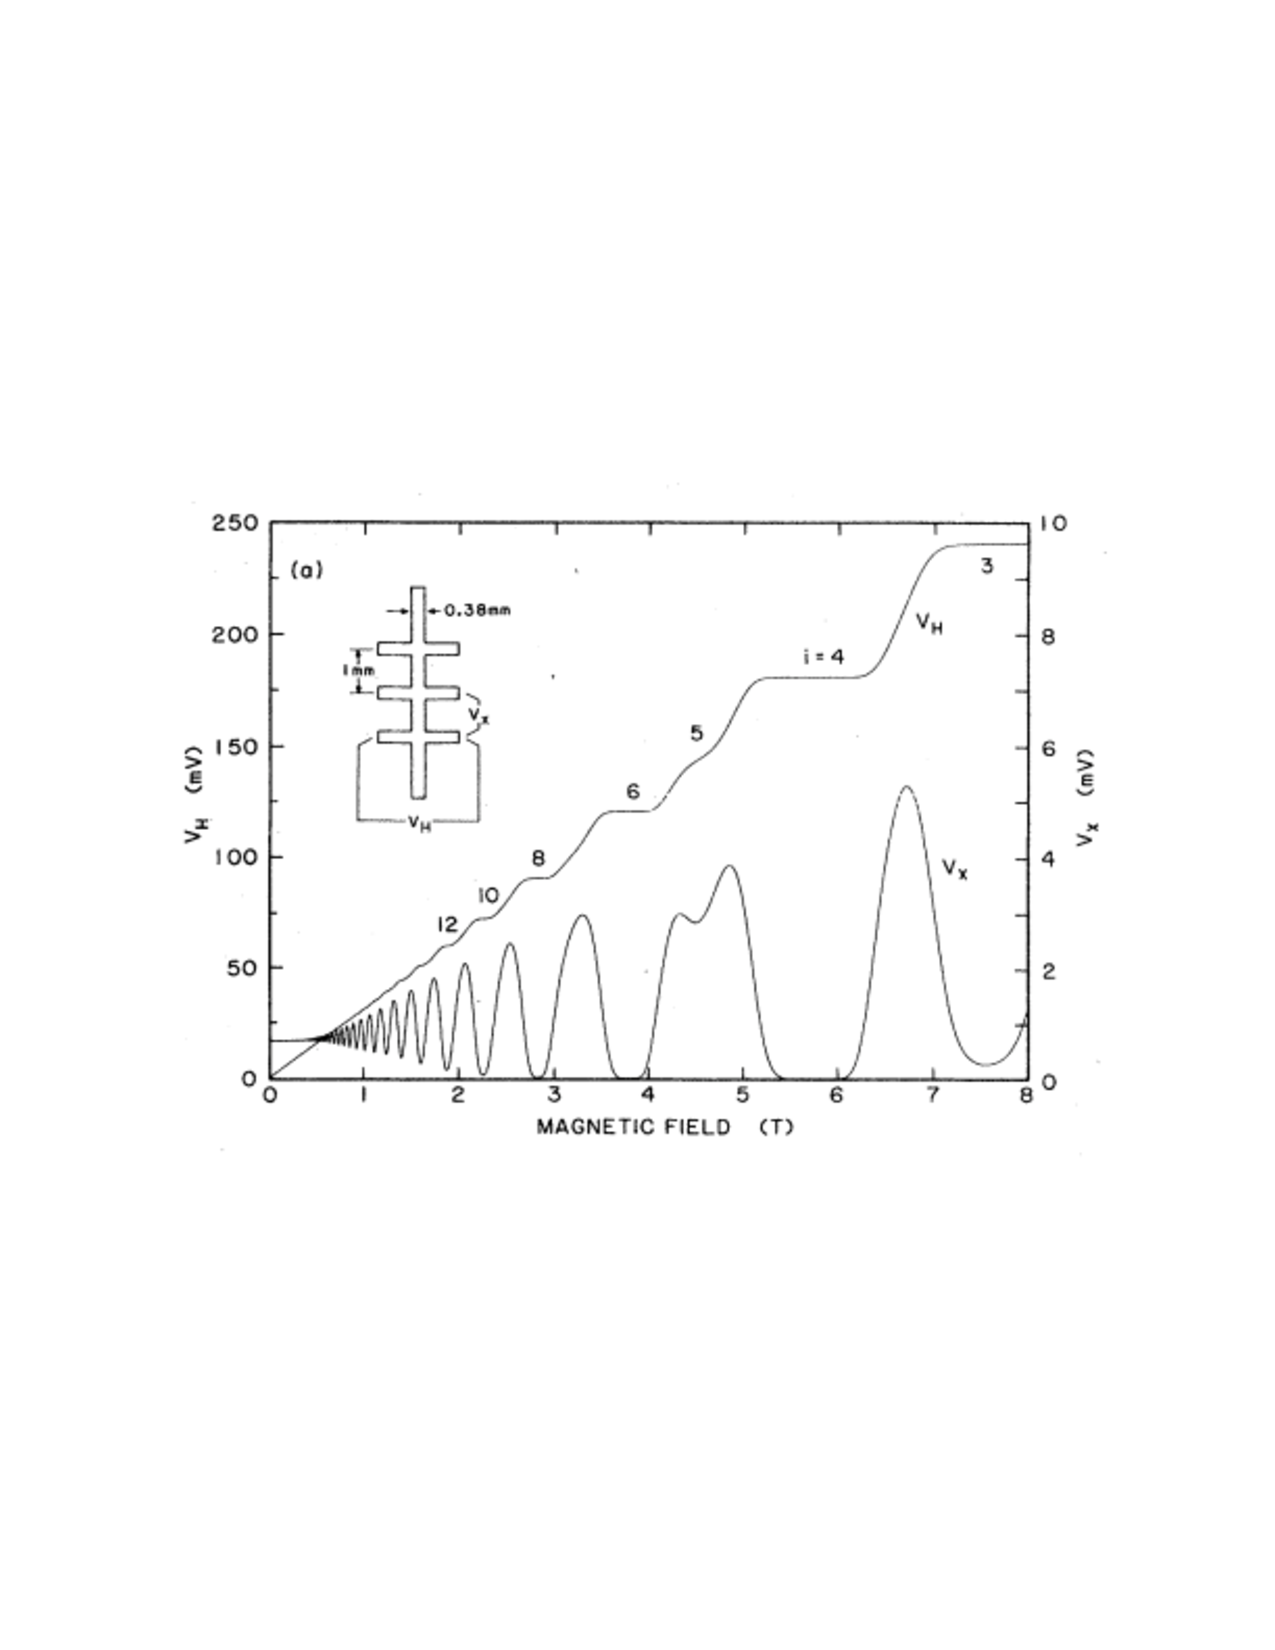
\includegraphics[width=10cm, angle=0]{ThesisCSULBLatexTemplate/figures/iqhe_plot_permission.pdf}
            \caption[The integer quantum Hall effect.]{The integer quantum Hall effect. Experimental data obtained from a GaAs heterostructure at $T=1.2$ K by Cage \textit{et al}. (1985). The Hall (transverse) resistivity sits on plateaus $\rho_{xy}=\frac{h}{e^2}\frac{1}{\nu}$ for a range of magnetic field values before suddenly jumping to the next plateau. The longitudinal resistivity, $\rho_{xx}$, vanishes at these plateaus before briefly spiking at each jump. Source: Reprinted with permission from Fig. 1 in  Ref. \cite{yennie}.}
            \label{iqhePlot}
            \end{center}
            \end{figure}
            
            These plateaus occur at
            \begin{equation} \label{iqhePlat}
            \rho_{xy}=\frac{h}{e^2}\frac{1}{\nu},
            \end{equation}
            where $\nu$ is measured to be an integer to one part per billion, and are centered around magnetic field strengths
            \begin{equation} \label{magFieldIqhe}
            B=\frac{h\rho}{\nu e}=\frac{\rho}{\nu}\phi_0.
            \end{equation}
            At low magnetic field strengths, the classical Hall effect is observed. However, when the electrons on the edges of the sample cannot complete their full cyclotron orbits, we often think of them as semiclassically bouncing around along the edges. This quenches the longitudinal resistance until the magnetic field reaches values where the edge orbits can be completed. At these magnetic field values, the Hall resistance jumps to a new plateau because the filling factor has decreased by one since the increased LL spacing has pushed the highest occupied LL above the Fermi energy~\cite{tong}. We can now explore what it means to be at a fractional filling factor.

        \subsection{Fractional Quantum Hall Effect}\label{ssec:fractQuantHallEff}\\
		
            Physicists found that as they decreased the sample disorder by trying other materials, lowering the temperature, and increasing the magnetic field strength, new plateaus in the Hall resistance became prominent. In 1982, Tsui \textit{et al}. were provided with a pure enough GaAs/AlGaAs semiconductor heterostructure sample to observe a plateau in the Hall resistivity at $\nu=1/3$ \cite{tsui}. Since then, over 70 rational fraction filling factors, $\nu=p/q$ for $p,q\in\mathbb{N}$, have been measured. A plot of this fractional quantum Hall effect (FQHE) can be seen in Fig. \ref{fqhePlot}.
		
		\begin{figure}[H]
            \begin{center}
            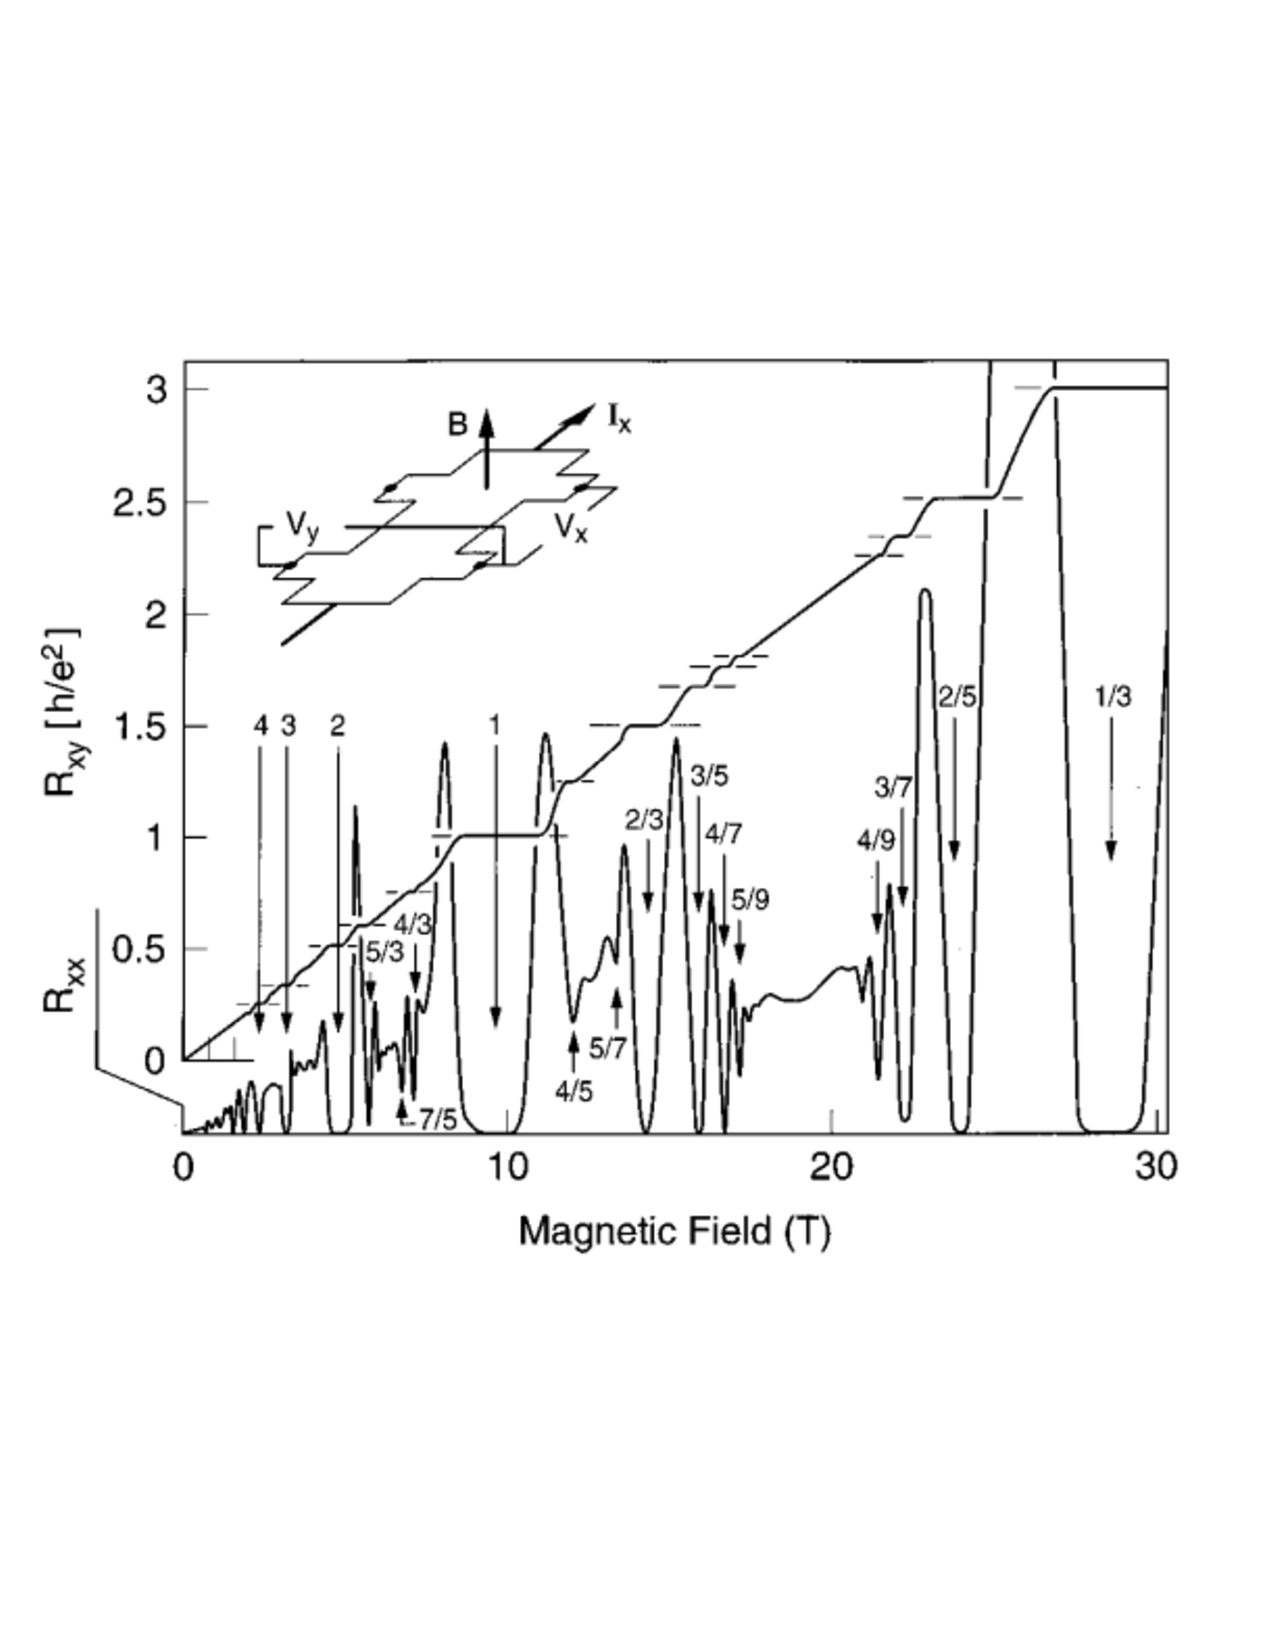
\includegraphics[width=10cm, angle=0]{ThesisCSULBLatexTemplate/figures/fqhe_plot.pdf}
            \caption[The fractional quantum Hall effect.]{The fractional quantum Hall effect. Experimental data obtained from a GaAs/AlGaAs heterostructure at $T=85$ mK by Eisenstein \textit{et al}. (1990). Like in the IQHE, the longitudinal resistance spikes at plateaus in the Hall resistance at $\rho_{xy}=\frac{h}{e^2}\frac{1}{\nu}$. However, this takes place at magnetic field strengths that correspond to rational fraction filling factors $\nu=\frac{p}{q}$, where $p,q\in\mathbb{N}$. Source: Reprinted with permission from Fig. 1 in Ref. \cite{stormer}.} 
            \label{fqhePlot}
            \end{center}
            \end{figure}
            
            As discussed in the previous section, the IQHE can be understood theoretically as an effect propagated by free electrons confined to two dimensions in a strong magnetic field, but Laughlin worked out that the Coulomb interactions between electrons must be taken into account to model the FQHE. It is then a many-body problem with Hamiltonian
            \begin{eqnarray}
                H = \sum_i \frac{\mathbf{\Pi}_i^2}{2m_b} + \sum_{i<j} \frac{e^2}{\epsilon l_B |\mathbf{r}_i-\mathbf{r}_j|} + \sum_i U(\mathbf{r}_i) + g\mu_B \mathbf{B}\cdot\mathbf{S},
            \end{eqnarray}
            where $\epsilon$ is the dielectric constant of the background material, $\mathbf{r}_i$ is the position of the $i^{th}$ electron, $U(\mathbf{r}_i)$ is a single particle potential (e.g. a confining potential), $g$ is the Land\'e g-factor, $\mu_B$ is the effective Bohr magneton, and $\mathbf{S}$ is the total spin of the electrons in the system. If we neglect $U(\mathbf{r}_i$), which amounts to a constant energy shift, and assume the electrons are fully polarized by the strong magnetic field, then the Hamiltonian becomes 
            \begin{eqnarray}
                H &=& \sum_i \frac{\hbar\omega_B}{2}(n_i + 1) + \sum_{i<j} \frac{e^2}{\epsilon l_B |\mathbf{r}_i-\mathbf{r}_j|}\;.
            \end{eqnarray}
            The kinetic energy term has vanished and the highest occupied LL is only fractionally filled for a rational fraction filling factor $\nu$. The electrons in the fractionally filled LL are degenerate, requiring a full solution of their Coulomb interactions - providing a difficult challenge for theorists. For these calculations, numerical approaches are used, including exact diagonalization of finite sized systems, Monte Carlo (MC) methods, and more recently, the density matrix renormalization group (DMRG).
            
            Laughlin published the following wave function for the ground state at filling factor $\nu=1/m$:
            \begin{equation}\label{eqn:one_over_m_wavefnx}
            \Psi_{1 / m}=\prod_{j<k}\left(z_{j}-z_{k}\right)^{m} \mathrm{e}^{-\frac{1}{4} \sum_{i}\left|z_{i}\right|^{2}},
            \end{equation}
            where $m$ is an odd integer to preserve antisymmetry and $z_j=x_j-iy_j$ are the coordinates of the j$^{th}$ electron in the complex plane using the symmetric gauge, $\mathbf{A} = B(-y,x,0)/2$. Through a series of arguments, he showed that this state, $\Psi_{1/m}$, describes a uniform density incompressible ground state with a finite energy gap which would experimentally manifest as a plateau in the Hall resistance at $\rho_{xy} = h/e^2(1/m)$. In addition, he worked out that the low energy excitations of these states have an electric charge of magnitude $e/m$ \cite{jain}.
            These excitations also obey Abelian fractional statistics, which can be found in the continuous range  between Fermi-Dirac and Bose-Einstein statistics \cite{laughlin}. The experimental demonstration of non-Abelian fractional statistics, which might occur in systems such as the FQHE at $\nu=5/2$ in GaAs heterostructures, could be the key step in building a topologically protected quantum computer \cite{nayak}. To explain filling factors other than those coming from Laughlin's wavefunction, however, we require composite fermion theory.
    		
\section{Composite Fermions}\label{sec:compFerm}

	Understanding the strongly-interacting electron problem directly proved to be difficult, but in 1989 Jain noticed that if the numbers on the plot of the FQHE (Fig.~\ref{fqhePlot}) were erased, it would be indistinguishable from the plot of the IQHE (Fig.~\ref{iqhePlot}). He used this insight to successfully  reformulate the FQHE in terms of noninteracting quasiparticles called composite fermions (CFs). The rest of this section will provide a brief introduction to this concept that follows from Jain's textbook \textit{Composite Fermions}~\cite{jain}.
	
	In CF theory, strongly-interacting electrons at filling factor $\nu$ in the lowest Landau level (LLL) are recast as functions of noninteracting (or weakly interacting) CFs that occupy Landau-like $\Lambda$ levels at CF filling factor $\nu^*$. The relationship between the electron and CF filling factors is given by
	\begin{equation} \label{compFermFill}
    \nu=\frac{\nu^*}{2p\nu^*\pm1},
    \end{equation}
    where $p\in\mathbb{N}_0$ and the minus sign in the denominator occurs when the effective magnetic field vector points opposite the external magnetic field vector. The CF wavefunction is given by
    \begin{equation} \label{compFermEigFunct}
    \Psi_\nu=\mathcal{P}_{LLL}\prod_{j<k}(z_j-z_k)^{2p}\Phi_{\nu^*},
    \end{equation}
    where $\Phi_{\nu^*}$ is the noninteracting electron wave function and $\mathcal{P}_{LLL}$ projects the state onto the lowest Landau level. CFs are the bound state between the noninteracting electrons in $\Phi_{\nu^*}$ and the $2p$ quantum vortices attached to them by the Jastrow factor,
    \begin{equation}\label{eqn:jastr_fact}
    \prod_{j}\mathcal{J}^p_j=\prod_{j<k}(z_j-z_k)^{2p}.
    \end{equation}
    
    The Berry phase of the attached vortices cancel the Aharanov-Bohm phase that arises as the CFs move about in the presence of an external magnetic field. Therefore, CFs exist in the reduced effective magnetic field $B^*$ at the mean-field level, 
    \begin{equation} \label{compFermMagnField}
    B^*=B-2p\rho\phi_0,
    \end{equation}
    where the electron and CF density $\rho$ is the same. If $\nu^*=n$ for $n\in\mathbb{N}$, it is reasonable to expect an energy gap to exist due to the $n$ filled $\Lambda$-levels, and therefore the CFs would manifest as plateaus centered around $B^*=(\rho/\nu^*)\phi_0$, analogous to the IQHE for electrons. This would then correspond to the FQHE of electrons for electron filling factor
    \begin{eqnarray}
        \nu = \frac{n}{2pn\pm 1},
    \end{eqnarray}
    which is precisely the values for most experimentally observed FQHE plateaus. 
    
    The energy expectation value for a FQH system at electron filling factor $\nu$ is 
    \begin{equation} \label{compFermEigEn}
    E_\nu=\frac{\braket{\Psi_\nu|\sum_{j<k}\frac{1}{r_{jk}}|\Psi_\nu}}{\braket{\Psi_\nu|\Psi_\nu}}+V_{el-bg}+V_{bg-bg}, 
    \end{equation}
	where $V_{el-bg}$ is the electron-background interaction energy, $V_{bg-bg}$ is the background-background interaction energy, and we are assuming there is a uniformly positively charged background such that the charge of the system is neutralized. The CF energy gaps are calculated via the CF-exciton ($\Delta$) dispersion. Excitons are CF-quasiparticle and CF-quasihole pairs created by the promotion of a CF to an unoccupied $\Lambda$ level. They are calculated as the difference between the ground state energy and the lowest energy of the state with a given total angular momentum, $L$. The CF-rotons ($\Delta_r$) are the minima of the exciton dispersion and can be measured experimentally via inelastic Raman scattering. The transport gap ($\Delta_t$), also referred to as the activation energy in the literature, is the energy required to create a quasiparticle and quasihole pair separated far enough to move independently, therefore contributing to transport. It converges to a constant value as the number of electrons increases, which can be measured experimentally via the longitudinal resistance as a function of the temperature. A schematic diagram of the exciton dispersion can be seen in Fig. \ref{transpGapDisp}. There exist energies above the line drawn on the plot, but we are only interested in visualizing the gap from the ground state to the lowest energy excitation at each wave vector $kl=L/\sqrt{Q}$. Analytical calculations of FQH energies require reformulating the problem in terms of Haldane pseudopotentials, which we will discuss in the next section.

    \begin{figure}[h]
    \begin{center}
    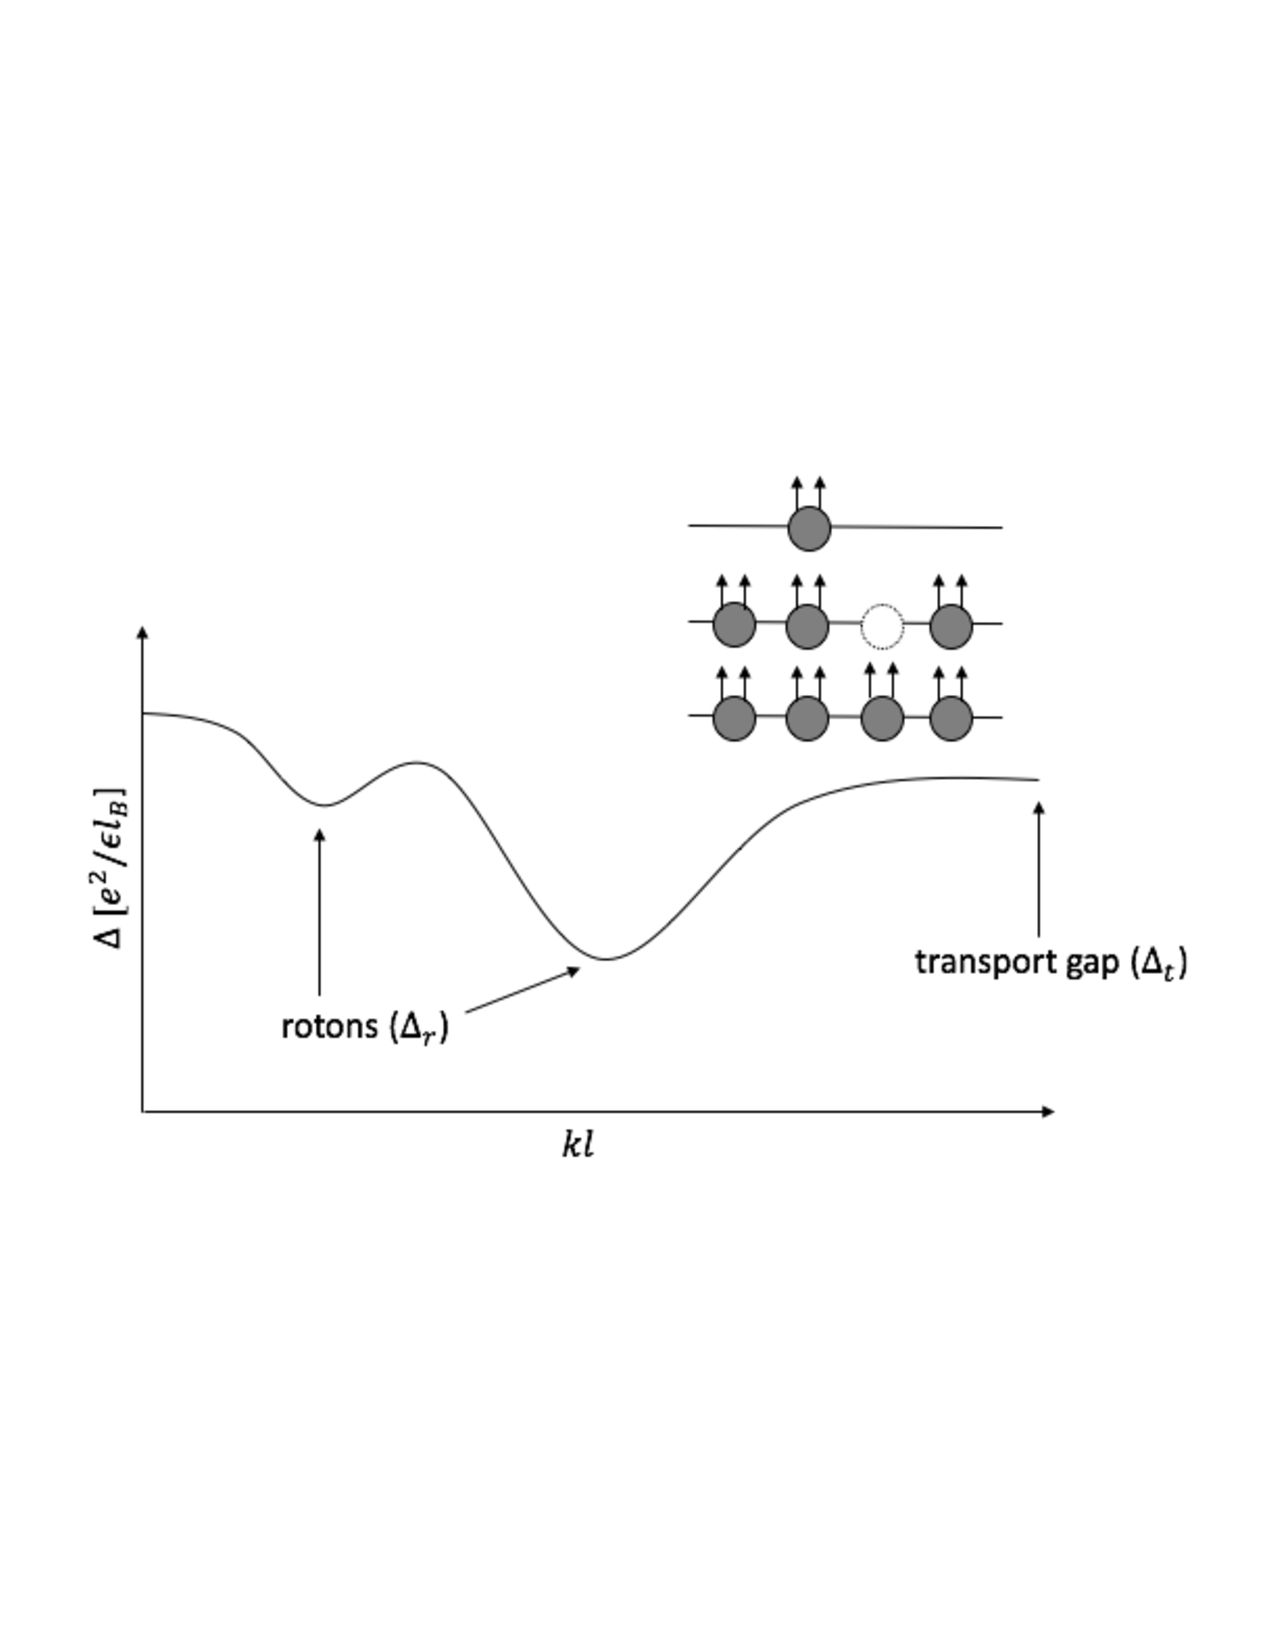
\includegraphics[width=10cm, angle=0]{ThesisCSULBLatexTemplate/figures/cf_exciton_drawing.pdf}
    \caption[The low energy composite fermion-exciton dispersion.]{The low energy composite fermion-exciton dispersion. Excitons ($\Delta$) are created by promoting a CF to an unoccupied $\Lambda$ level (inset). The rotons ($\Delta_r$) are the local minima of the dispersion. At large wave vectors $kl$, the dispersion converges to the transport gap ($\Delta_t$), where the quasiparticle and quasihole pair are separated far enough to move independently. The plotted line represents the gap between the ground state and the lowest energy excitation for each wave vector.}
    \label{transpGapDisp}
    \end{center}
    \end{figure}

    \section{Haldane Pseudopotentials}\label{sec:haldPseud}
    The FQHE is a challenging many-body problem, requiring theorists to solve the fully interacting Hamiltonian 
    \begin{eqnarray}
        H &=& \sum_{i<j} \frac{e^2}{\epsilon l_B |\mathbf{r}_i-\mathbf{r}_j|}\;,
    \end{eqnarray}
    where we have neglected the kinetic energy term. In 1983, Haldane introduced a useful parameterization of the interacting FQHE Hamiltonian in terms of so-called Haldane pseudopotentials (PPs) \cite{haldane}. Very generally, the Hamiltonian can be rewritten as
    \begin{eqnarray}\label{HamPPexpand}
        H &=& \sum_{i<j} \frac{e^2}{\epsilon l_B |\mathbf{r}_i-\mathbf{r}_j|}\nonumber\\
        &=& \sum_m V^{(n)}_m \sum_{i<j} P_{ij}(m),
    \end{eqnarray}
    where $m$ is the relative angular momentum between the $i^{th}$ and $j^{th}$ electrons, $P_{ij}(m)$ is a projection operator for a state with relative angular momentum $m$, and $V^{(n)}_m$ are the Haldane pseudopotentials. The PP represents the interaction energy between two electrons confined to the $n^{th}$ LL with relative angular momentum $m$. They are a useful parameterization because, for a given interaction potential, they completely determine the problem and significantly simplify numerical approaches such as exact diagonalization.
    
    In this thesis, we utilize Haldane's spherical geometry where the two-dimensional plane is mapped to the boundary free surface of a sphere of constant radius $R=\sqrt{Q}l_B$. The perpendicular magnetic field becomes a radial magnetic field emanating from a magnetic monopole in its center with strength $Q$ (see Fig.~\ref{fig:haldSpher}). Mapping this problem to the spherical geometry mitigates complications that arise from edge effects. In 1976, Tai Tsun Wu and Chen Ning Yang solved for the wavefunction of a charged particle moving in the presence of a Dirac monopole \cite{wu}. The single particle eigenstates in the spherical geometry are the monopole harmonics
	\begin{equation} \label{monHarm}
    Y_{q,n,m}(\Omega)=N_{qnm}2^{-m}(1-x)^{\frac{-q+m}{2}}(1+x)^{\frac{q+m}{2}}P_{q+n-m}^{-q+m,q+m}(x)e^{i(q-m)\phi},
    \end{equation}
    where $N_{qnm}$ is the normalization coefficient
    \begin{equation} \label{monHarmNormCo}
    N_{qnm}=\left(\frac{(2q+2n+1)}{4\pi}\frac{(q+n-m)!(q+n+m)!}{n!(2q+n)!}\right)^{1/2},
    \end{equation}
    the total flux through the sphere is $2q\phi_0$ for $2q\in\mathbb{Z}$, $m=-q-n,-q-n+1,...,q+n$ are the degenerate states in the $n^{th}$ LL, $l=q+n$ is the single particle angular momentum, $x=cos\theta$, and $P^{\alpha,\beta}_\gamma$ are the Jacobi polynomials \cite{bible}. 
    
    \begin{figure}[h]
    \begin{center}
    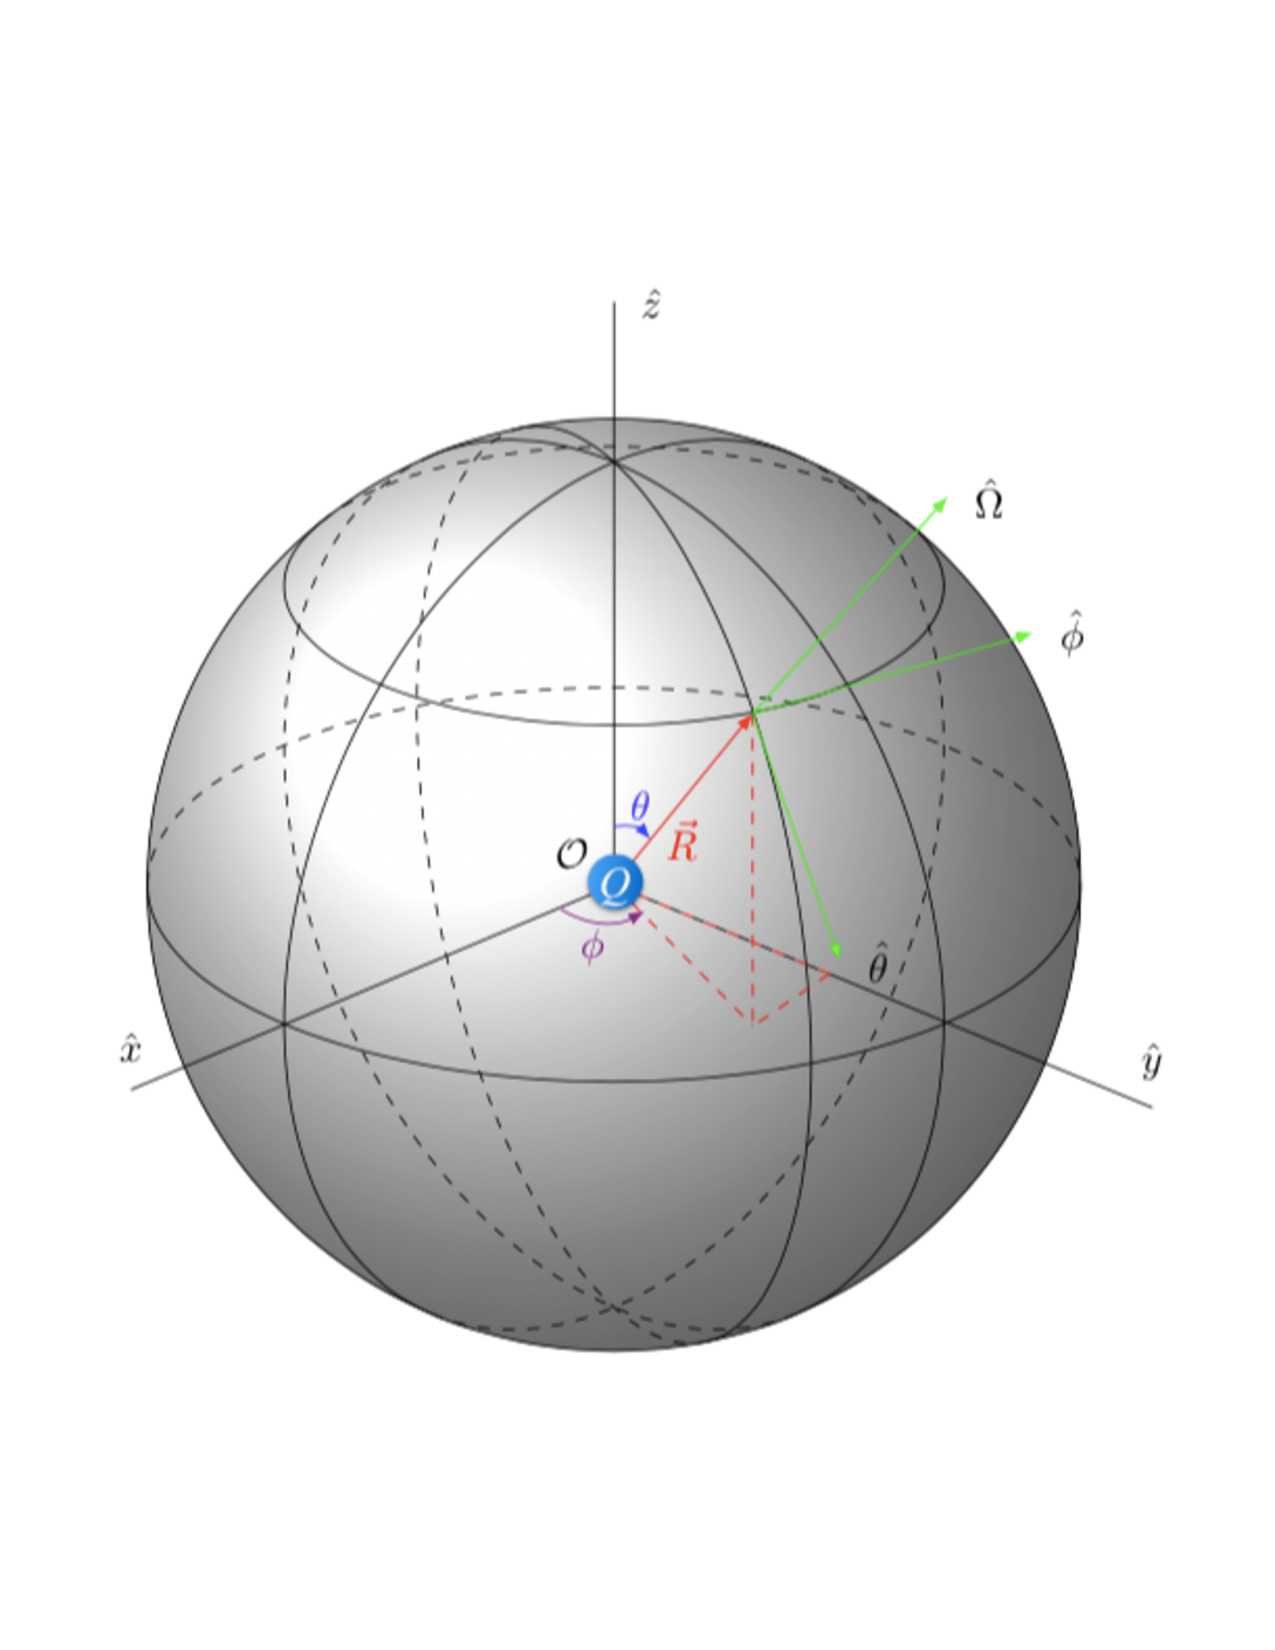
\includegraphics[width=10cm, angle=0]{ThesisCSULBLatexTemplate/figures/haldane_sphere_thesis.pdf}
    \caption[The Haldane sphere.]{The Haldane sphere. The 2D electron gas is mapped to the surface of a sphere of radius $R=\sqrt{Q}l_B$ to mitigate complications arising from edge effects. The perpendicular magnetic field emanates from a magnetic monopole of strength $Q$ in the sphere's center. Source: Reprinted with permission from Fig. 1 in  Ref.~\cite{arciniaga}.}
    \label{fig:haldSpher}
    \end{center}
    \end{figure}
    
    \vspace{4pt} % keep uniform double spacing below caption
    
    The MC code we use to calculate the exciton dispersion requires a real space potential to calculate the interaction energies between electrons on the Haldane sphere. We will be incorporating realistic material effects into the PPs, which have no explicit form in real space since the mapping between real space and the spherical geometry is not bijective. Therefore, we need to use an effective potential in real space that can reflect the changes realistic effects make to the bare Coulomb PP. In her 2013 doctoral dissertation, Rachel Wooten published a scheme for mapping an effective real space potential to a PP in the spherical geometry. The $n^{th}$ LL PP,
    \begin{equation} \label{wootPpNthLl}
    V_{l,Q}=\braket{Q,l,l;L,M|V(|r_{12}|)|Q,l,l;L,M},
    \end{equation}
    is given in Coulomb units by
    \begin{equation} \label{wootPp}
    V_{l,Q}(L)=\frac{1}{\sqrt{Q}}\sum_{k=0}^{2l}V_k(-1)^{2Q+L}(2l+1)^2
    \begin{Bmatrix}
    L & l & l\\
    k & l & l
    \end{Bmatrix}
    \begin{pmatrix}
    l & k & l\\
    -Q & 0 & Q
    \end{pmatrix}
    ^2,
    \end{equation}
    where $l=|Q|+|n|$ is the single-particle angular momentum, $L=2l-m$ is the two-body relative angular momentum in the spherical geometry,
    \begin{equation} \label{wootPpVk}
    V_k=\frac{1}{2}\int_0^\pi V(r_{12})P_k(\cos\theta)\sin\theta d\theta,
    \end{equation}
    $V(r_{12})$ is the effective two-dimensional interaction, $P_k(cos\theta)$ are the Legendre polynomials, the curly bracket matrix contains Wigner's 6-j symbols, and the round bracket matrix contains Wigner's 3-j symbols~\cite{wooten}. Plugging an effective interaction $V(r_{12})$ into this expression yields its corresponding PP in the spherical geometry as a function of the relative angular momentum, $V_{l,Q}(L)$. We work with PPs in the spherical geometry since it is more amenable to the addition of realistic effects. However, solving for the energies in terms of PPs in the spherical geometry via exact diagonalization requires an expansion of Slater determinant basis states which makes calculations impractical for systems with larger than $\sim10$ electrons. For this reason, we instead approximate the energies via a variational Monte Carlo (MC) method (see Sec.~\ref{ssec:montCarlInt} for more details). This MC method, however, requires a real space potential, so we incorporate realistic effects into our energy calculations by mapping the real space potential (to be used in the MC calculation) to a realistic effect-incorporated PP in the spherical geometry via Wooten's method.
    
    A popular choice in the literature for a real space potential for MC calculations is the Park potential. Park $\textit{et al.}$ investigated the mysterious even-denominator FQH state at $\nu=5/2$, where the CF filling factor of the first-excited LL is $\nu^*=1/2$. They devised the following effective interaction in the LLL (in units of $e^2/\epsilon l_B$) to produce the same PPs as the Coulomb interaction in the first-excited LL:
    \begin{equation} \label{parkPot}
    V_{eff}(r)=\left(\frac{1}{r}+a_1e^{-\alpha_1r^2}+a_2r^2e^{-\alpha_2r^2}\right)\left[\frac{e^2}{\epsilon l_B}\right],
    \end{equation}
    where the distance $r$ is in units of effective magnetic length $l_{B^*}=(\hbar/eB^*)^{1/2}$, the fitting parameters $\{a_1,a_2,\alpha_1,\alpha_2\}$ are calculated by fitting the first four significant PPs exactly, $\epsilon$ is the dielectric constant of the background material, and $l_B=\sqrt{\frac{\hbar}{eB}}$ is the magnetic length at actual electron filling factor $\nu$. The first four significant PPs are those for which $m\in\{1,3,5,7\}$ - they are odd because the many-body wavefunction has to be fully anti-symmetric under particle exchange for fermions, and since in the planar geometry $m$ is directly proportional to the chord distance between electrons $r$ in the potential $V(r)$, the first four sample the strongest Coulomb interactions \cite{park}. We will be fitting a modified version of the Park potential to PPs that incorporate realistic effects into the spherical geometry via Wooten's formula (see Sec.~\ref{ssec:realSpaceEffPot}). The first realistic effect we want to benchmark our method against, LLM, can be quenched in the $B\rightarrow\infty$ limit for GaAs/AlGaAs semiconductor heterostructures, but not in the material graphene, which we will discuss in the next section.

    \section{Graphene}\label{sec:graph}
    In 2004, Novoselov \textit{et al}. developed a simple way to isolate graphene, an atomically-thin hexagonal carbon lattice, using regular adhesive tape \cite{novoselov}. The next year, Novoselov \textit{et al}. found that the electrons and holes in graphene obey a linear dispersion, appropriate for massless particles. In this case, the Fermi velocity $\nu_F$ is approximately $10^6$ m/s \cite{novoselov2005}. In 2009, both Du \textit{et al}. and Bolotin \textit{et al}. separately manufactured pure enough samples of suspended graphene to observe the FQHE at $\nu=1/3$ \cite{du,bolotin}. The next year, Skachko \textit{et al}. measured a clear plateu in the Hall resistivity at $\nu=1/3$ in temperatures ranging from 2 K to up to 20 K in a 12 T external magnetic field. The charge carrier density, which corresponds to the filling factor $\nu$, can be adjusted in graphene at a constant magnetic field via the gate voltage $V_g$ \cite{skachko}. In 2015, Amet \textit{et al}. demonstrated the FQHE in other filling factors of graphene, $\nu=\frac{p}{2p\pm1}$, where $p$ is an integer less than or equal to 5 \cite{amet}. A plot of the FQHE in graphene can be seen in Fig. \ref{fqheGraph}.
	
    \begin{figure}[H]
    \begin{center}
    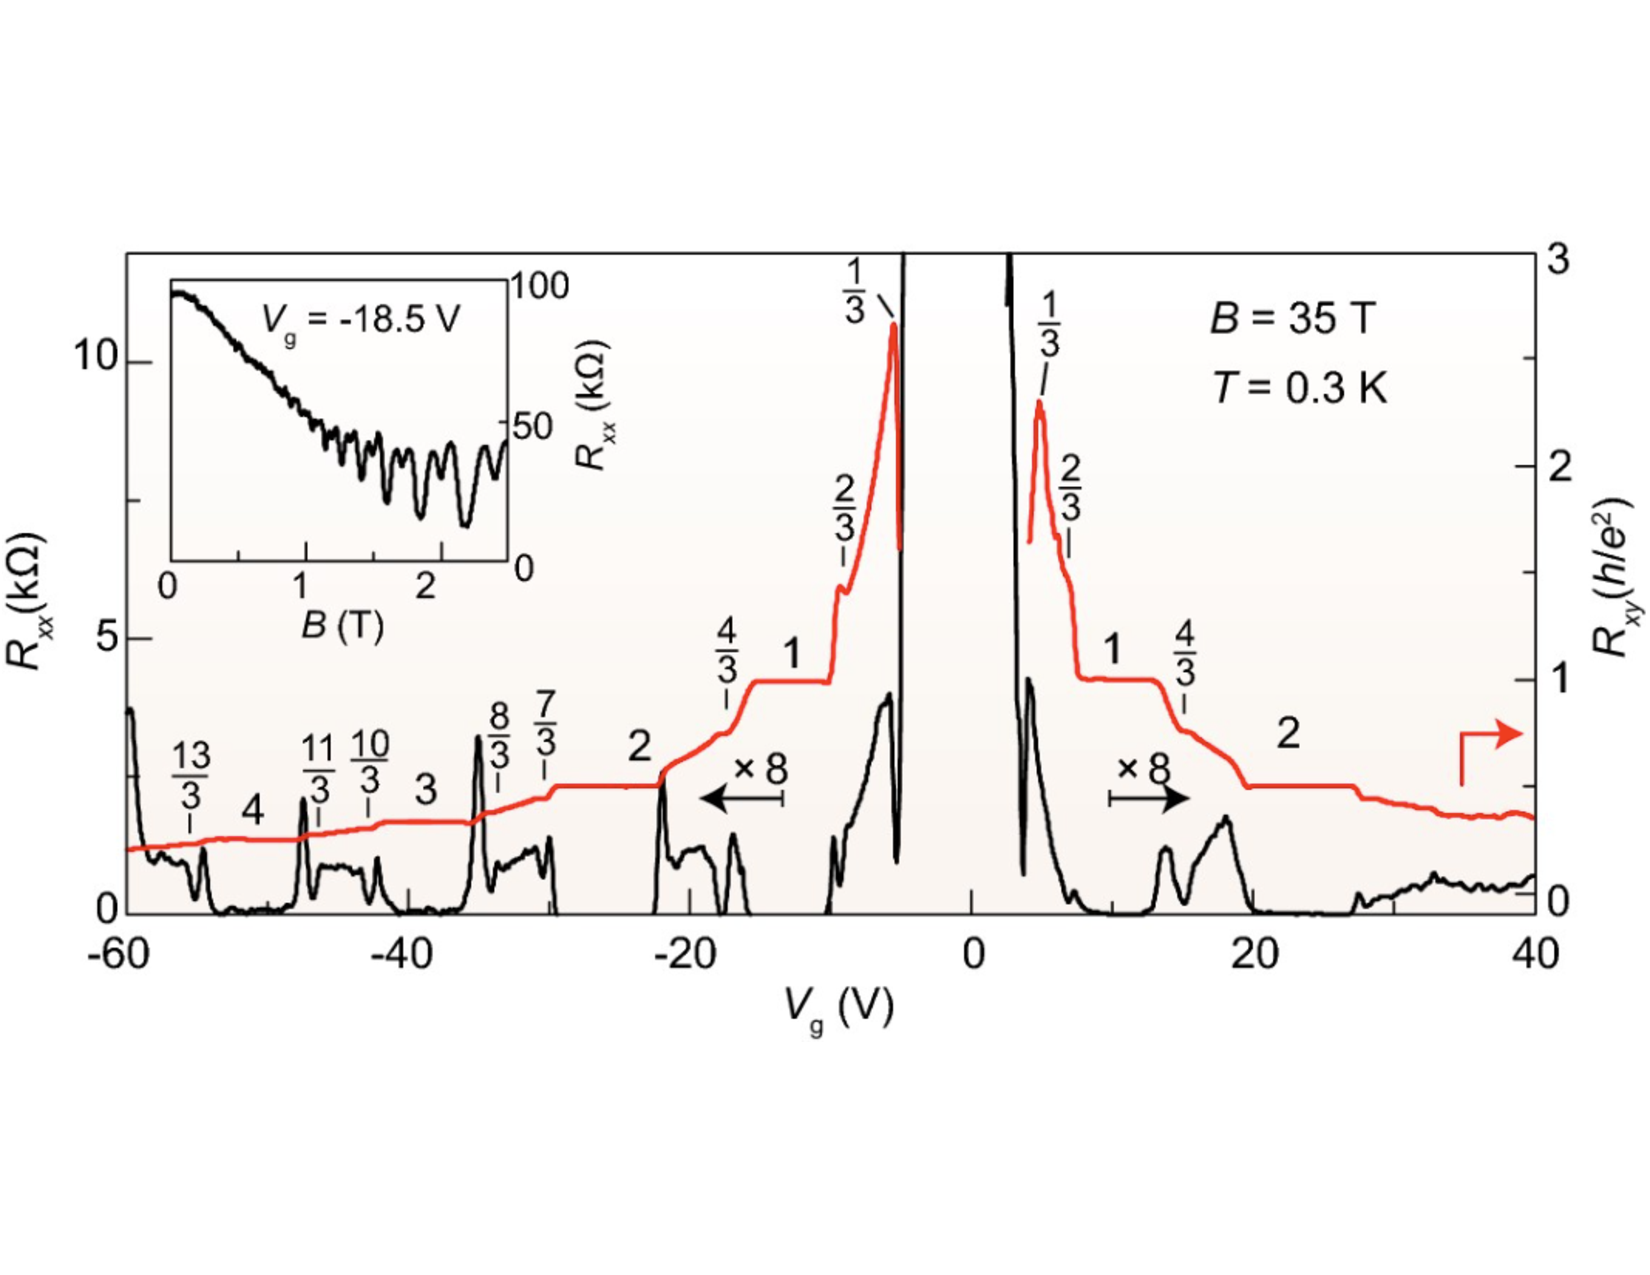
\includegraphics[width=10cm, angle=0]{ThesisCSULBLatexTemplate/figures/fqhe_graphene.pdf}
    \caption[The FQHE in graphene.\vspace{-12pt}]{The FQHE in graphene. Experimental data obtained from graphene at $T=0.3$ K by Dean \textit{et al.} (2011). In graphene, the gate voltage $V_g$ can be used to adjust the filling factor $\nu$ at a constant magnetic field strength (i.e. $B=35$ T). Source: Adapted from Fig. 13 in Ref. \cite{lin}.}
    \label{fqheGraph} 
    \end{center}
    \end{figure}
    
    For free electrons in graphene, there are two Fermi points $K$ and $K^\prime$, each with a two-fold band degeneracy (from the $A$ and $B$ sublattice). The continuum Hamiltonian for one pseudospin component is 
    \begin{eqnarray}
    H &=& \nu_F \mathbf{\sigma}\cdot \mathbf{\Pi}\\
    &=& \nu_F \begin{pmatrix}
    0 & \Pi_x - i \Pi_y\\
    \Pi_x + i\Pi_y & 0
    \end{pmatrix}\;,
    \end{eqnarray}
    where $\mathbf{\sigma} = (\sigma_1, \sigma_2, \sigma_3)$ are the Pauli matrices and $\mathbf{\Pi}$ is the canonical momentum defined in Eq.~\ref{eq:can_mom}. The following is adapted from Refs.~\cite{arciniaga, apalkov, goerbig, toke, nomura, Toke2007}. Reintroducing the ladder operators from before, we get the Hamiltonian
    \begin{eqnarray}
    H&=& \nu_F\frac{\hbar\sqrt{2}}{l_B} \begin{pmatrix}
    0 & a \\
    a^\dagger & 0
    \end{pmatrix}\;.
    \end{eqnarray}
    The standard way to solve this Hamiltonian is to instead consider its square, 
    \begin{eqnarray}
    H^2 &=& \nu_F^2\frac{2\hbar^2}{l_B^2} \begin{pmatrix}
    aa^\dagger & 0 \\
    0 & a^\dagger a
    \end{pmatrix}\;,
    \end{eqnarray}    
    which is simpler because $[a,a^\dagger]=1$ and $a^\dagger a=n$ is the number operator. The eigenfunctions of $H^2$ can be found to be 
    \begin{eqnarray}
        \psi_{nm}(x,y) = \frac{(\sqrt{2})^{\delta_{n0}}}{\sqrt{2}}
        \begin{pmatrix}
        -\mathrm{sgn}(n) i \eta_{|n|-1,m}(x,y) \\
        \eta_{|n|m}(x,y)
        \end{pmatrix},
    \end{eqnarray}
    where $\eta_{nm}(x,y)$ are the single-particle eigenfunctions of the quadratic energy dispersion for massive fermions. Since $[H,H^2]=0$, the two Hamiltonians share common eigenfunctions and the energy spectrum can be found to be
    \begin{eqnarray} \label{eqn:graphSpectr}
        E_n &=& \frac{\hbar \nu_F}{l_B} \sqrt{2|n|}\;.
    \end{eqnarray}
    This different spectrum and eignenstate structure augments the PPs for the FQHE in graphene. However, it can essentially be expressed in terms of combinations of the massive electron result for semiconductor heterostructures given in Eq.~\ref{wootPpNthLl} (see Arciniaga and Peterson for more details~\cite{arciniaga}). The linear electron dispersion and energy spectrum given in Eq.~\ref{eqn:graphSpectr} create a unique LL structure for graphene. The spacing between energy eigenvalues in a GaAs/AlGaAs semiconductor heterostructure remained constant as a function of the cyclotron energy $\hbar\omega_B$, but in graphene, the LLs clump together as the space between their energies decreases at larger LL indices $n$. This creates problems for theorists using traditional methods to calculate the CF exciton dispersion for graphene because there is then no magnetic field strength that can quench the effects of Landau level mixing, which we will discuss in the next section.
	
	\subsection{Landau Level Mixing} \label{ssec:landLevMix}
	    In 2006, T\ifmmode \mbox{\H{o}}\else \H{o}\fi{}ke \textit{et al}. calculated the transport gaps for FQH states of graphene at filling factor $\nu\in\{1/3,2/5\}$ \cite{toke}. However, theoretical predictions for measurable gaps have not yielded acceptable agreement with experiment. It is typical for these calculations to ignore Landau level mixing (LLM), an effect that arises when Coulomb interactions push electrons into higher LLs, or alternatively, holes into lower LLs. It is characterized by the parameter $\kappa$, the ratio of the Coulomb energy to the cyclotron energy. One of the factors that makes these calculations unique for graphene is its linear, as opposed to parabolic, electron dispersion. This prevents the suppression of LLM by a sufficiently strong magnetic field via the following relation from Ref. \cite{peterson2014}:
        \begin{equation} \label{kappGraph}
        \kappa = 
        \begin{cases} 
        \frac{e^2/\epsilon l_B}{\hbar\omega_B} \sim \frac{2.5}{\sqrt{B[\text{tesla}]}}, & \text{GaAs semiconductor} \\
        \frac{e^2/\epsilon l_B}{\hbar\nu_F/l_B} = \frac{e^2}{\epsilon\hbar\nu_F}=\frac{2.2\text{ (Kelvin)}}{\epsilon}, & \text{graphene.}
        \end{cases}
        \end{equation}
        The experimental value of $\kappa$ depends on the substrate the sample rests upon. For a suspended graphene sample $~{\kappa}\approx2.2$, for graphene on a SiO$_2$ substrate $~{\kappa}\approx0.9$, and for a boron nitride substrate $~{\kappa}\approx0.5-0.8$ \cite{peterson}.
	    
	    Peterson \textit{et al}. developed a scheme for incorporating LLM effects into PPs via the following Hamiltonian \cite{peterson2014}:
        \begin{equation} \label{hamHaldSphere}
        \begin{split}
        H(\kappa) & = \sum_{i<j}V_{eff}(\kappa,|\mathbf{r}_i-\mathbf{r}_j|)+\sum_{i<j<k}V_{3body}(\kappa,\mathbf{r}_i,\mathbf{r}_j,\mathbf{r}_k) \\
        & = \sum_\alpha V_\alpha^{(2)}(N,\kappa)\sum_{i<j}\hat{P}_m(m_{ij}) + \sum_\beta V_\beta^{(3)}(N,\kappa)\sum_{i<j<k}\hat{P}_{ijk}(m_{ijk}),
        \end{split}
        \end{equation}
        where $\hat{P}_m(m_{ij})$ projects electrons $i$ and $j$ onto their respective angular momentum state $m_{ij}$, $\hat{P}_{ijk}(m_{ijk})$ projects electrons $i$, $j$, and $k$ onto $m_{ijk}$, and $V_\alpha^{(2)}(N,\kappa)$ and $V_\beta^{(3)}(N,\kappa)$ are the $\kappa$ dependent two and three-body effective PPs, respectively. For LLs $n\ge1$, LLM generates particle-hole symmetry breaking three-body terms, but in the LLL (which we confine ourselves to in this thesis), the three-body terms in Eq.~\ref{hamHaldSphere} vanish due to this symmetry \cite{peterson}. 
        
        In 2016, Arciniaga \textit{et al}. calculated perturbative corrections to the two-body PPs in the LLL, $\delta V^{(n=0)}_{2l-m}$, such that the corrected two-body PPs are given by
        \begin{equation} \label{potLlm}
        V^{(0)}_{2l-m,2body}(\kappa) = V^{(0)}_{2l-m} + \kappa\delta V^{(0)}_{2l-m},
        \end{equation}
        where $V^{(0)}_{2l-m}$ is the two-body bare Coulomb PP in the LLL \cite{arciniaga}. Then, in his master's thesis, Hernandez found that increasing $\kappa$ increases the ground state energy for $\nu\in\{1/3,2/5,3/7\}$ \cite{uriel}. We are interested in how the LLM parameter $\kappa$ affects the rotons and transport gaps since they are readily measurable by experiment. We want to develop a systematic way to efficiently incorporate realistic effects, like LLM in graphene, into calculations of these energy gaps. We will be perturbatively adding the two-body PP corrections in the LLL due to LLM calculated by Arciniaga \textit{et al}. to the bare Coulomb PPs via Eq. \ref{potLlm}. We will then use Wooten's method (Eq.~\ref{wootPp}) to fit an effective real space potential to the corrected PPs for use in the Monte Carlo code, which we will discuss in the next chapter.

\singlespacing